\section{Transformando los tractogramas al espacio $LogOdds$}

En la secci\'on anterior presentamos algunos de los inconvenientes 
te\'oricos del m\'etodo propuesto por Moreno-Dominguez. Los mismos eran el
clustering de vectores colineales; la relaci\'on entre la m\'etrica y el
\textit{linkage} y la alta complejidad algor\'itmica. En esta secci\'on
proponemos una forma de solucionarlos haciendo uso de la funci\'on 
\textit{logit}. La funci\'on \textit{logit} permite convertir vectores
provenientes de distribuciones discretas al espacio $LogOdds$. El 
espacio $LogOdds$ es un espacio vectorial. Esto quiere decir que es 
cerrado respecto a la suma y la multiplicaci\'on por escalares. A 
continuaci\'on presentamos la transformaci\'on $logit$ en detalle; luego
mostramos como esto permite solventar los problemas presentados y mejorar 
la complejidad algor\'itmica del $clustering$. \\

\subsection{Transformaci\'on Logit}
\label{sec:logit}

Sea $P_M$ el espacio de una distribuci\'on discreta para $M$ etiquetas: 

$$P_M = \left\{  p | p = (p_1,\dots p_n) \in (0,1)^M , \sum{p_i} = 1 \right\}$$

La funci\'on \textit{logit}:$P_M \rightarrow R^{M-1}$ define una
transformaci\'on entre el espacio $P_M$ y un espacio vectorial $R^{M-1}$.
A este espacio vectorial se lo denomina $LogOdds$. Dados los vectores 
$Q \in P^M$ y $S \in R^{M-1}$:

$$S_i = logit(Q_i) = log\left(\frac{Q_i}{Q_M}\right)$$

Para el caso de $M=2$ el espacio de origen es la distribuci\'on Bernoulli
discreta. Podemos ver en la ecuaci\'on \ref{eq:logit} su expresi\'on 
anal\'itica y en la figura \ref{fig:dominio} su representaci\'on gr\'afica.

\begin{figure}[h!]

\begin{minipage}[b]{0.45\textwidth}

    \begin{equation}
    \vspace{2.85cm}
        \label{eq:logit}
    logit(p) = log\left(\frac{p}{1-p}\right)
    \end{equation}
\end{minipage} ~
\hfill
\begin{minipage}[b]{0.45\textwidth}
    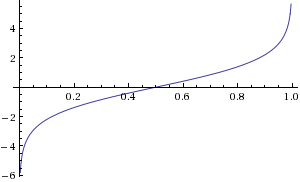
\includegraphics[width=\textwidth]{img/logit.png}
    \caption{Representaci\'on gr\'afica de la funci\'on $logit$. La misma
             nos permite transformar los tractogramas a un espacio
             vectorial. }
    \label{fig:dominio}
\end{minipage} ~

\end{figure}  

Trabajar en un espacio vectorial nos asegura que la suma y la 
multiplicaci\'on por escalares est\'an contenidos en el mismo espacio.
Pohl et al. \cite{Pohl2007} utilizan esta propiedad para realizar
operaciones lineales sobre mapas probabil\'isticos. A su vez, muestran
que la suma y multiplicaci\'on por escalares en el espacio $LogOdds$ 
poseen un significado en el espacio de la distribuci\'on. La suma en el
espacio $LogOdds$ representa una multiplicaci\'on normalizada en el
espacio de origen:

$$ p_1 \oplus p_2 = logit^{-1} ( logit(p_1) + logit(p_2) ) = 
   \frac{1}{ p_1 \cdot p_2 } (p1_1 p2_1, \dots, p1_n p2_n) $$

donde $p_1$ y $p_2$ son vectores provenientes de una misma distribuci\'on y
$X_1 \cdot X_2$ es el producto interno entre $X_1$ y $X_2$. Multiplicar
por un escalar $\alpha$ en el espacio de $LogOdds$ equivale a exponenciar
la distribuci\'on por $\alpha$ y normalizarla:

$$ \alpha \otimes p = logit^{-1} ( logit(p_1) \alpha ) = 
   \frac{1}{\sum p_{i}^{\alpha}}(p_1^{\alpha}, \dots, p_n^{\alpha})  $$

\subsection{Modificando el algoritmo de clustering}
\label{sec:modificandoClustering}

Veamos como modificar el agrupamiento de tractogramas utilizando la
funci\'on $logit$. Asumiendo que cada voxel $v$ de un tractograma proviene 
de la variable aleatoria binaria:

$$X_v= \textrm{``La semilla est\'a conectada con el voxel v''}$$
 
Es posible transformar el tractograma aplicando la funci\'on 
\textit{logit} en cada uno de sus voxels. El resultado es un vector donde
cada coordenada se encuentra en el espacio $LogOdds$. M\'as a\'un, las
operaciones lineales entre los mismos voxels en distintos tractogramas 
est\'an definidas. Esto nos permite usar la m\'etrica euclidiana como
funci\'on de similitud en \textit{Agglomerative Hierarchical Clustering}.\\

Transformar de espacio los tractogramas y cambiar la funci\'on de
similitud posee varias ventajas. Para empezar permite agrupar
correctamente vectores colineales. La figura \ref{fig:3logit} muestra el
resultado de aplicar este m\'etodo a los vectores de la figura
\ref{fig:3clusters}. Podemos apreciar que las tres poblaciones se
encuentran correctamente separadas y bien definidas.\\

\begin{figure}[h!]

\centering
\begin{minipage}[b]{0.85\textwidth}
    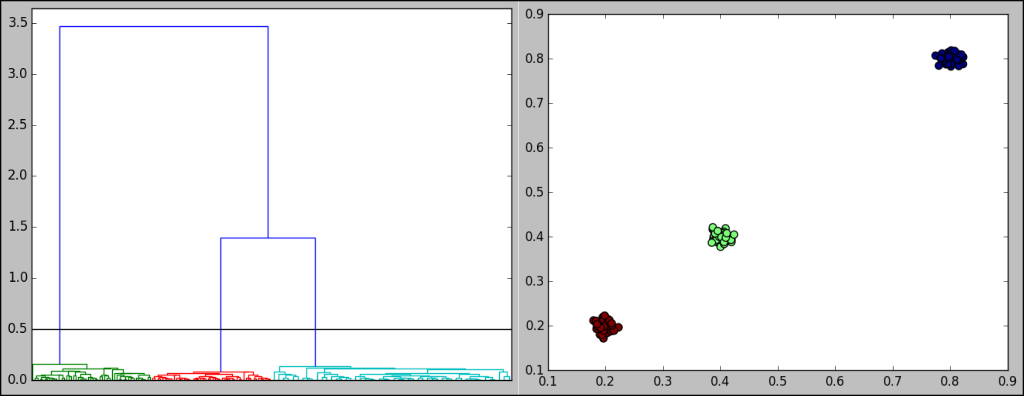
\includegraphics[width=\textwidth]{img/3pop_logit.png}
    
    \caption{Clustering resultado de utilizar nuestro m\'etodo para 
             agrupar los vectores. Los tres $clusters$ fueron separados
             correctamente.}
    \label{fig:3logit}
\end{minipage} ~

\end{figure}  

Otra ventaja es la buena relaci\'on m\'etrica-\textit{linkage}. Por
definici\'on el centroide es el centro de masa de los clusters. Esto
quiere decir que es el punto que minimiza la distancia euclidiana entre
los clusters que lo componen. Por ende, el centroide caracteriza bien el
punto medio de los vectores en el espacio eucl\'ideo. \\

Finalmente, nuestro m\'etodo tambi\'en permite mejorar la complejidad
algor\'itmica. El algoritmo \textit{Agglomerative Herarchical Clustering}
une en cada iteraci\'on dos $clusters$, calcula un representante de estos
y luego computa su distancia al resto. Usar la m\'etrica euclidiana junto
con el \textit{linkage} centroide es posible simplificar estos pasos. \\

\begin{equation}
\label{eq:lyw}
d(i \cup j,k) = \alpha_i d(i,k) + \alpha_j d(i,k) + \beta d(i,j) + \gamma | d(i,k) - d(j,k) |
\end{equation}

\begin{equation}
\label{eq:lyw2}
\alpha_i = \frac{|i|}{|i|+|j|} \hspace{0.5cm}
\alpha_j = \frac{|j|}{|i|+|j|} \hspace{0.5cm}
\beta = -\frac{|k|}{|i|+|j|+|k|} \hspace{0.5cm}
\gamma = 0
\end{equation}


La formula de Lance y Williams (ecuaci\'on \ref{eq:lyw}) permite computar
las distancias entre $clusters$ {\bf sin compararlos expl\'icitamente}. 
Para el m\'etodo centroide los par\'ametros son las relaciones de la 
ecuaci\'on \ref{eq:lyw2}. Usar esta formula reduce significativamente la
complejidad. Cada iteraci\'on pasa a costar $O(c^2)$ en  vez de $O(c^2 m)$,
siendo $c$ la cantidad de clusters y $m$ la longitud de los mismos. Dadas
$s$ semillas iniciales, la complejidad temporal total del 
\textit{clustering} es $O(s^3)$.  En la secci\'on 
\ref{sec:complejidad_moreno} se ve que usando la distancia coseno era 
$O(s^3 m)$, siendo $m$ la longitud de los tractogramas. El no comparar 
expl\'icitamente los clusters permite no tener que mantenerlos en memoria.
Esto reduce significativamente la complejidad temporal. Solo es necesario
almacenar la matriz de distancias entre clusters. Esto tiene un costo
espacial total de $O(s^2)$. La secci\'on \ref{sec:complejidad_moreno} 
muestra que usando la distancia coseno esta complejidad era $O(sm +s^2)$.
Recordemos que en el contexto en que estamos utilizando este algoritmo
$m>>s$. Por lo tanto, este resultado implica una gran reducci\'on en la
complejidad del algoritmo. \\
